\documentclass{article}

\usepackage[utf8]{inputenc}
\usepackage[margin=3cm]{geometry}
\usepackage{graphicx}
\usepackage{minted}
\usepackage{xcolor}
\usepackage{hyperref}
\usepackage{caption}

\hypersetup{colorlinks,linkcolor=,urlcolor=blue}
\usemintedstyle{friendly}
\definecolor{bg}{rgb}{0.95,0.95,0.95}

\title{Lab 05: A ``gentle'' Introduction to Decision Trees in R}
\author{Andrés Oswaldo Calderón Romero, PhD.}
\date{\today}

\begin{document}

\maketitle

\section{Introduction}
Decision trees are a type of Supervised Machine Learning where the data is continuously split according to specific parameters. They are highly interpretable, mimicking human decision-making processes.

\section{The Play\_Tennis Dataset}
We are using the \href{https://drive.google.com/file/d/1oxH5tVJkF2An3O5m80sbYNexTnE1xaeF/view?usp=sharing}{\texttt{play\_tennis\_dataset.csv}}. This dataset predicts whether to play tennis based on the \textbf{Outlook}, \textbf{Temperature}, \textbf{Humidity}, and \textbf{Wind}.

\subsection{Building the Model in R}
The \texttt{rpart} package is the standard tool for creating Recursive Partitioning trees in R.

\begin{listing}[H]
\begin{minted}[
frame=lines,
framesep=2mm,
baselinestretch=1.2,
bgcolor=bg,
fontsize=\footnotesize
]{r}
# Load necessary libraries
library(rpart)
library(rpart.plot)

# Load the dataset
tennis_data <- read.csv("play_tennis_dataset.csv")

# Remove the 'Day' column (unnecessary for prediction)
tennis_data$Day <- NULL

# Build the model with custom controls to force depth
model <- rpart(PlayTennis ~ .,
               data = tennis_data,
               method = "class",
               control = rpart.control(cp = 0,        # No minimum improvement
                                       minsplit = 2,  # Split even with 2 samples
                                       maxdepth = 2)) # Limit to 2 levels deep
# View the basic structure
print(model)
\end{minted}
\caption{Model construction using \texttt{rpart}.}
\end{listing}

\subsection{Mathematical Foundation: Entropy}
Decision trees split the data at the point that maximizes ``purity''. This is often measured using \textbf{Entropy}.

$$H(S) = - \sum_{i=1}^{c} p_i \log_2(p_i)$$

By calculating the Entropy before and after a split, we determine the \textbf{Information Gain}. The variable with the highest Information Gain becomes the node.

\subsection{Visualizing the Results}
The \texttt{rpart.plot} package provides a ``ready-to-publish'' visualization of the tree logic.  We will get a tree as shown figure \ref{fig:play_tennis_tree}.

\begin{listing}[H]
	\begin{minted}[
	frame=lines,
	framesep=2mm,
	bgcolor=bg,
	fontsize=\footnotesize
	]{r}
	# Visualize the decision-making process
	rpart.plot(model,
			type = 2,
			extra = 101,
			under = TRUE,
			box.palette = "GnYlRd",
			main = "Play Tennis: 2-Level Decision Logic")
	\end{minted}
	\caption{Visualizing the decision tree.}
\end{listing}

\begin{figure}
 \centering
 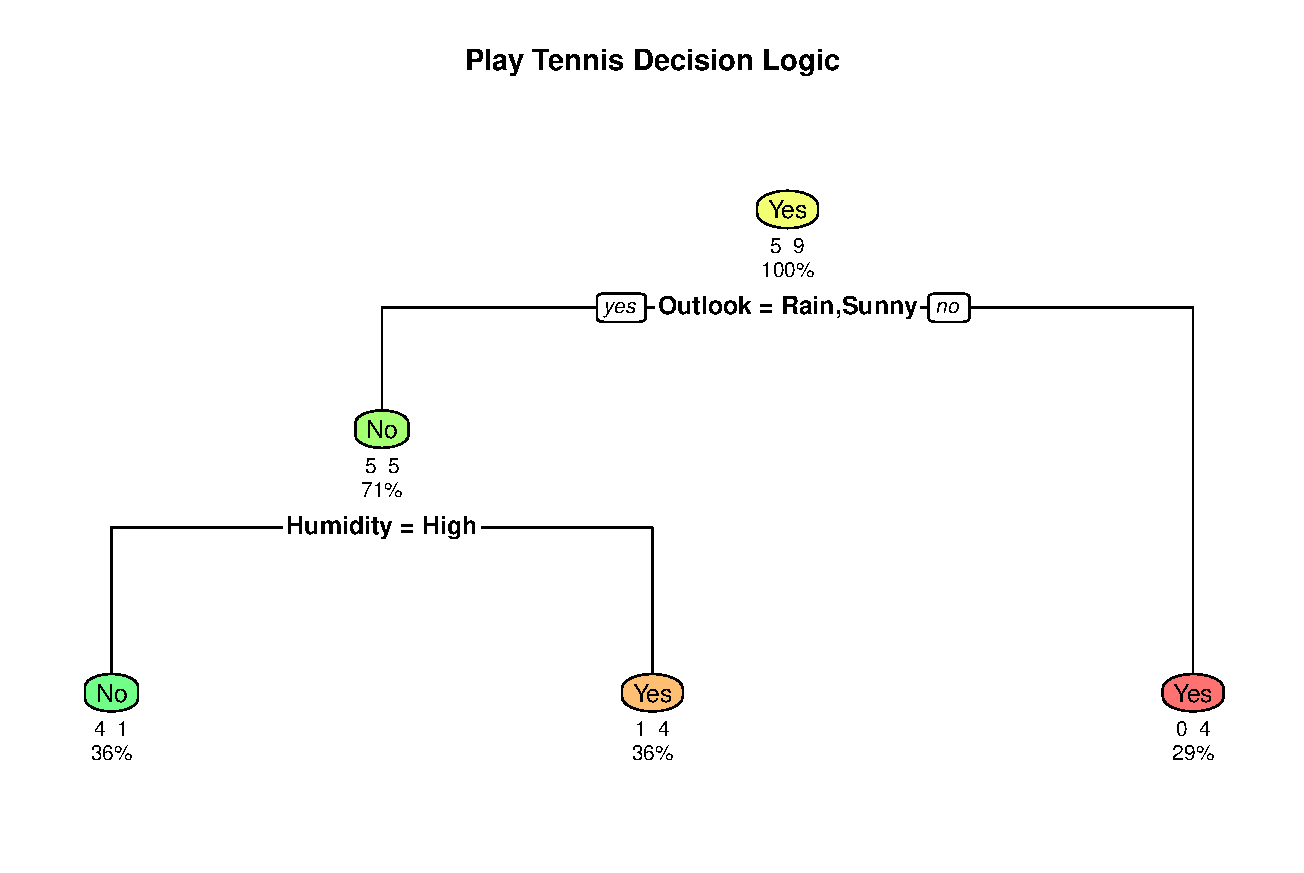
\includegraphics[width=0.75\textwidth]{figures/play_tennis_tree}
 \caption{Play tennis classification tree.}
 \label{fig:play_tennis_tree}
\end{figure}

\subsection{Predicting New Data}
Finally, we can pass new observations to our model to get a ``Yes'' or ``No'' prediction.

\begin{listing}[H]
	\begin{minted}[
		frame=lines,
		framesep=2mm,
		bgcolor=bg,
		fontsize=\footnotesize
	]{r}
# Create a new weather scenario
new_weather <- data.frame(
Outlook = "Rain",
Temperature = "Mild",
Humidity = "High",
Wind = "Weak"
)

# Generate prediction.  Output should be: 'Prediction for the new day: No'
res <- predict(model, new_weather, type = "class")
cat("Prediction for the new day:", as.character(res))

	\end{minted}
	\caption{Predicting with the trained model.}
\end{listing}

\subsection{Summary of Parameters}
\begin{itemize}
    \item \textbf{Level 0 (Root)}: Usually splits on the most important variable (e.g., Outlook).
    \item \textbf{Level 1}: Secondary decisions based on the remaining entropy (e.g., Humidity or Wind).
    \item \textbf{Overfitting Note}: While forcing a tree to be deeper makes it look better, be careful! On small datasets, a deep tree might learn ``noise'' rather than actual patterns.
\end{itemize}

%%%%%%%%%%%%%%%%%%%%%%%%%%%%%%%%%%%%%%
\section{The Advertisement Dataset} \label{sec:ad}
We will build a classifier to predict if a person purchases a product based on their \textit{Age} and \textit{Estimated Salary} using the \texttt{rpart} package.  This exercise was taken at ``\textit{Decision Tree Classifiers in R Programming}'' tutorial from \href{https://www.geeksforgeeks.org}{GeeksforGeeks}\footnote{@GeeksforGeeks, Sanchhaya Education Private Limited, All rights reserved.  2026. ``\textit{Decision Tree Classifiers in R Programming}''. Available at: \url{https://www.geeksforgeeks.org/r-language/decision-tree-classifiers-in-r-programming/}. Accessed:  April 2026.} portal.

\subsection{Installing and Loading Packages}
Load the necessary libraries for model construction, data splitting, and visualization.

\begin{minted}[bgcolor=bg, breaklines]{r}
# run the below line just one time...
# install.packages(c("rpart", "rpart.plot", "caTools", "ggplot2", "dplyr"))

library(rpart)
library(rpart.plot)
library(caTools)
library(ggplot2)
library(dplyr)
\end{minted}

\subsection{Loading the Dataset}
The dataset contains advertising expenditures across media channels and their impact on sales.  You can download the dataset \href{https://drive.google.com/file/d/1uFJtgMXrU2W9v6Pp6V1AsN8FSvicEgI5/view?usp=sharing}{here}.

\begin{minted}[bgcolor=bg]{r}
# Loading the Advertisement dataset
dataset <- read.csv("Advertisement.csv")
head(dataset, 10)

    User.ID Gender Age EstimatedSalary Purchased
1  15624510   Male  19           19000         0
2  15810944   Male  35           20000         0
3  15668575 Female  26           43000         0
4  15603246 Female  27           57000         0
5  15804002   Male  19           76000         0
6  15728773   Male  27           58000         0
7  15598044 Female  27           84000         0
8  15694829 Female  32          150000         1
9  15600575   Male  25           33000         0
10 15727311 Female  35           65000         0
\end{minted}

\subsection{Preparing the Data}
Encode the target variable as a factor and split the data into training (75\%) and testing (25\%) sets.

\begin{minted}[bgcolor=bg]{r}
# Convert target variable to factor
dataset$Purchased <- factor(dataset$Purchased, levels = c(0, 1))

# Splitting dataset
set.seed(42)
split <- sample.split(dataset$Purchased, SplitRatio = 0.75)
training_set <- subset(dataset, split == TRUE)
test_set <- subset(dataset, split == FALSE)
\end{minted}

\subsection{Feature Scaling}
Normalize numerical features so that they share the same scale.

\begin{minted}[bgcolor=bg, breaklines]{r}
# Normalize numerical features
training_set[c("Age", "EstimatedSalary")] <- scale(training_set[c("Age", "EstimatedSalary")])
test_set[c("Age", "EstimatedSalary")] <- scale(test_set[c("Age", "EstimatedSalary")])

head(training_set, 5)
   User.ID Gender        Age EstimatedSalary Purchased
3 15668575 Female -1.1010703      -0.8561205         0
5 15804002   Male -1.7902649       0.1299869         0
6 15728773   Male -1.0026140      -0.4078899         0
7 15598044 Female -1.0026140       0.3690432         0
8 15694829 Female -0.5103322       2.3412580         1

head(test_set, 5)
    User.ID Gender        Age EstimatedSalary Purchased
1  15624510   Male -1.7695949       -1.268692         0
2  15810944   Male -0.3588566       -1.240511         0
4  15603246 Female -1.0642257       -0.197828         0
14 15704987   Male -0.6233700       -1.296872         0
22 15736760 Female  0.6991972       -0.423273         1
\end{minted}

\subsection{Fitting the Classifier}
Train the recursive partitioning model on the training data.

\begin{minted}[bgcolor=bg, breaklines]{r}
# Fitting Decision Tree to the Training set
classifier <- rpart(formula = Purchased ~ Age + EstimatedSalary,
                    data = training_set,
                    method = "class")
\end{minted}

\subsection{Visualization}
Visualize how the decision tree partitions the predictor space.  Result appears in figure \ref{fig:ad_tree}.

\begin{minted}[bgcolor=bg, breaklines]{r}
# Decision tree
rpart.plot(classifier,
           type = 2,
           extra = 101,
           under = TRUE,
           box.palette = "BlGnYl",
           main = "Ad Decision Logic")
\end{minted}

\begin{figure}
 \centering
 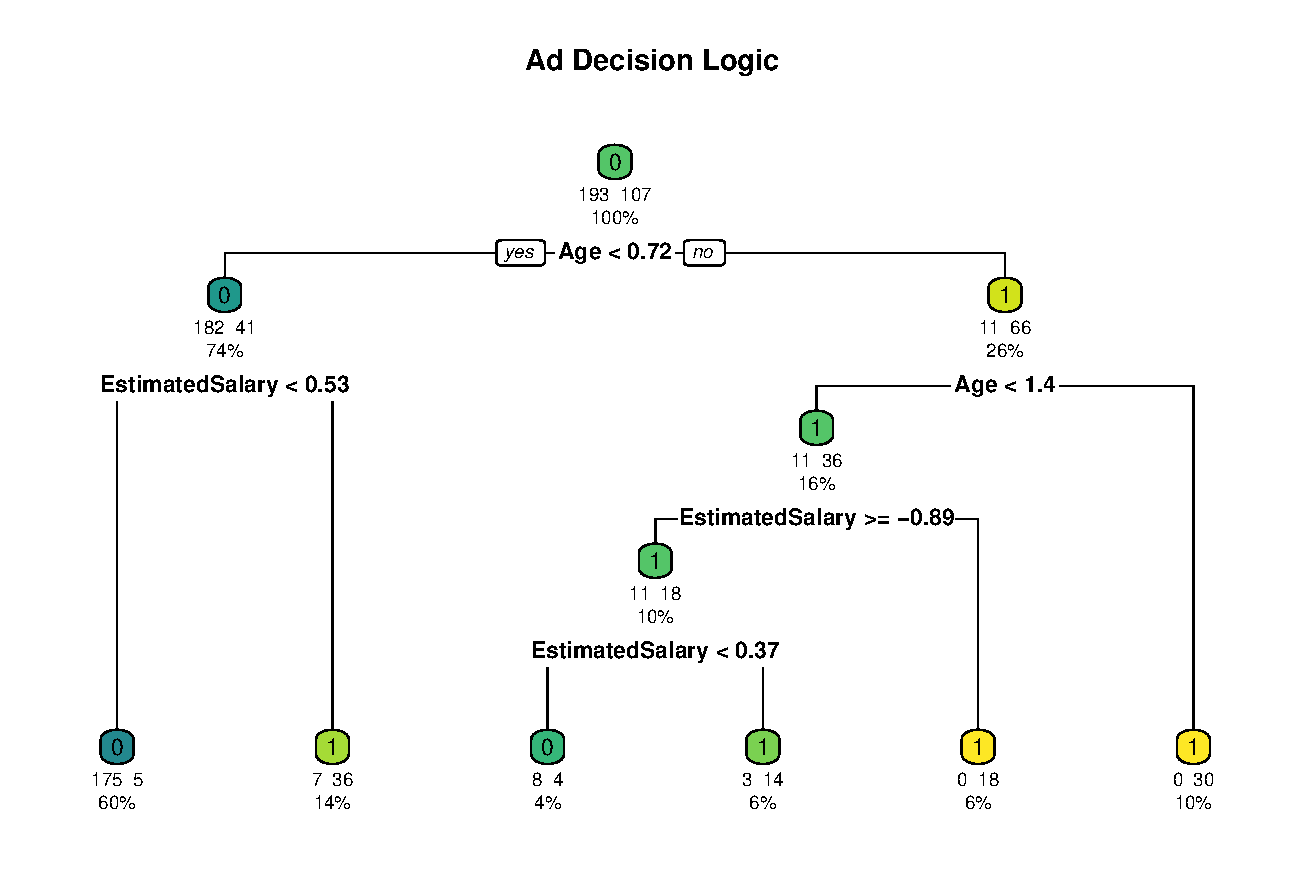
\includegraphics[width=0.75\textwidth]{figures/ad_tree}
 \caption{Ad classification tree.}
 \label{fig:ad_tree}
\end{figure}

\subsection{Model Evaluation}
After fitting the model, it is essential to measure its performance using a \textbf{Confusion Matrix} to calculate metrics like accuracy.

\subsubsection{Predicting Test Set Results}
Apply the model to the independent test set to generate predictions.

\begin{minted}[bgcolor=bg, breaklines]{r}
# Predicting the Test set results
y_pred <- predict(classifier, newdata = test_set[-5], type = "class")
\end{minted}

\subsubsection{Confusion Matrix and Accuracy}
Compare the predicted classes against actual values.  Figure \ref{fig:cm} shows the results.

\begin{minted}[bgcolor=bg, breaklines]{r}
# Creating the Confusion Matrix
cm <- table(test_set[, 5], y_pred)
print(cm)

# Accuracy calculation
accuracy <- sum(diag(cm)) / sum(cm)
print(paste("Model Accuracy: ", round(accuracy, 2)))
\end{minted}

\begin{figure}
 \centering
 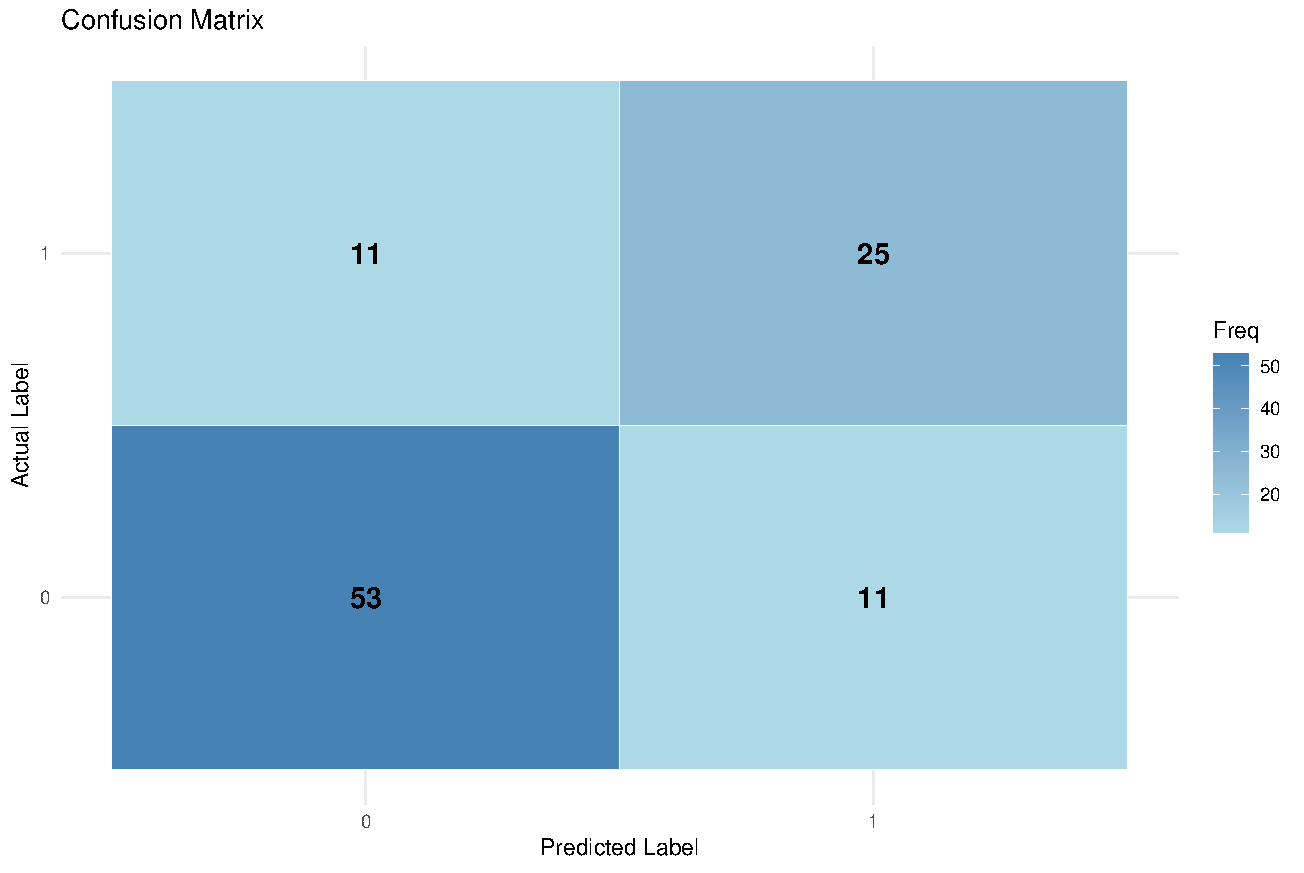
\includegraphics[width=0.75\textwidth]{figures/cm}
 \caption{Decision matrix.}
 \label{fig:cm}
\end{figure}

%%%%%%%%%%%%%%%%%%%%%%%%%%%%%%%%%%%%%%

\section{Autonomous Work}
\label{sec:autonomous}

In this section, you are required to replicate the decision tree implementation detailed in Section~\ref{sec:ad} using an alternative programming ecosystem. The goal is to demonstrate that while syntax varies, the underlying machine learning logic remains consistent across platforms.

You may select one of the following language-library combinations:

\begin{description}
    \item[Python] \texttt{scikit-learn} or \texttt{XGBoost} / \texttt{CatBoost}
    \item[Java] \texttt{Smile} or \texttt{Weka}
    \item[Julia] \texttt{DecisionTree.jl}
    \item[C++] \texttt{MLPACK} or \texttt{Dlib}
    \item[JavaScript / TypeScript:] \texttt{ml-cart} or \texttt{TensorFlow.js}
    \item[Rust] \texttt{SmartCore} or \texttt{Linfa}
\end{description}

\end{document}
